
%% Journal.tex
%% V0.1
%% 2019/11/16
%% by Edward Eisenberger
%%
%% This contains the content for the AES Dynamic S-Box Generation with
%% Diffie-Hellman Exchange for the IEEE journal paper.
\documentclass[journal]{IEEEtran}
% \documentclass[journal]{../sty/IEEEtran}

% *** MISC UTILITY PACKAGES ***
%\usepackage{ifpdf}
% Heiko Oberdiek's ifpdf.sty is very useful if you need conditional
% compilation based on whether the output is pdf or dvi.
% usage:
% \ifpdf
%   % pdf code
% \else
%   % dvi code
% \fi
% The latest version of ifpdf.sty can be obtained from:
% http://www.ctan.org/pkg/ifpdf
% Also, note that IEEEtran.cls V1.7 and later provides a builtin
% \ifCLASSINFOpdf conditional that works the same way.
% When switching from latex to pdflatex and vice-versa, the compiler may
% have to be run twice to clear warning/error messages.

% *** GRAPHICS RELATED PACKAGES ***
\ifCLASSINFOpdf
  \usepackage[pdftex]{graphicx}
  % declare the path(s) where your graphic files are
  \graphicspath{{../Graphics/PDF/}{../Graphics/EPS/}}
  % and their extensions so you won't have to specify these with
  % every instance of \includegraphics
  % \DeclareGraphicsExtensions{.pdf,.jpeg,.png}
\else
  % or other class option (dvipsone, dvipdf, if not using dvips). graphicx
  % will default to the driver specified in the system graphics.cfg if no
  % driver is specified.
  % \usepackage[dvips]{graphicx}
  % declare the path(s) where your graphic files are
  % \graphicspath{{../eps/}}
  % and their extensions so you won't have to specify these with
  % every instance of \includegraphics
  % \DeclareGraphicsExtensions{.eps}
\fi
% graphicx was written by David Carlisle and Sebastian Rahtz. It is
% required if you want graphics, photos, etc. graphicx.sty is already
% installed on most LaTeX systems. The latest version and documentation
% can be obtained at: 
% http://www.ctan.org/pkg/graphicx
% Another good source of documentation is "Using Imported Graphics in
% LaTeX2e" by Keith Reckdahl which can be found at:
% http://www.ctan.org/pkg/epslatex
%
% latex, and pdflatex in dvi mode, support graphics in encapsulated
% postscript (.eps) format. pdflatex in pdf mode supports graphics
% in .pdf, .jpeg, .png and .mps (metapost) formats. Users should ensure
% that all non-photo figures use a vector format (.eps, .pdf, .mps) and
% not a bitmapped formats (.jpeg, .png). The IEEE frowns on bitmapped formats
% which can result in "jaggedy"/blurry rendering of lines and letters as
% well as large increases in file sizes.
%
% You can find documentation about the pdfTeX application at:
% http://www.tug.org/applications/pdftex

% *** MATH PACKAGES ***
%
\usepackage{amsmath}
\usepackage{algorithm}
\usepackage[noend]{algpseudocode}
% A popular package from the American Mathematical Society that provides
% many useful and powerful commands for dealing with mathematics.
%
% Note that the amsmath package sets \interdisplaylinepenalty to 10000
% thus preventing page breaks from occurring within multiline equations. Use:
\interdisplaylinepenalty=2500
% after loading amsmath to restore such page breaks as IEEEtran.cls normally
% does. amsmath.sty is already installed on most LaTeX systems. The latest
% version and documentation can be obtained at:
% http://www.ctan.org/pkg/amsmath

% *** SPECIALIZED LIST PACKAGES ***
%
%\usepackage{algorithmic}
% algorithmic.sty was written by Peter Williams and Rogerio Brito.
% This package provides an algorithmic environment fo describing algorithms.
% You can use the algorithmic environment in-text or within a figure
% environment to provide for a floating algorithm. Do NOT use the algorithm
% floating environment provided by algorithm.sty (by the same authors) or
% algorithm2e.sty (by Christophe Fiorio) as the IEEE does not use dedicated
% algorithm float types and packages that provide these will not provide
% correct IEEE style captions. The latest version and documentation of
% algorithmic.sty can be obtained at:
% http://www.ctan.org/pkg/algorithms
% Also of interest may be the (relatively newer and more customizable)
% algorithmicx.sty package by Szasz Janos:
% http://www.ctan.org/pkg/algorithmicx

% *** ALIGNMENT PACKAGES ***
%
%\usepackage{array}
% Frank Mittelbach's and David Carlisle's array.sty patches and improves
% the standard LaTeX2e array and tabular environments to provide better
% appearance and additional user controls. As the default LaTeX2e table
% generation code is lacking to the point of almost being broken with
% respect to the quality of the end results, all users are strongly
% advised to use an enhanced (at the very least that provided by array.sty)
% set of table tools. array.sty is already installed on most systems. The
% latest version and documentation can be obtained at:
% http://www.ctan.org/pkg/array

% IEEEtran contains the IEEEeqnarray family of commands that can be used to
% generate multiline equations as well as matrices, tables, etc., of high
% quality.

% *** SUBFIGURE PACKAGES ***
%\ifCLASSOPTIONcompsoc
%  \usepackage[caption=false,font=normalsize,labelfont=sf,textfont=sf]{subfig}
%\else
%  \usepackage[caption=false,font=footnotesize]{subfig}
%\fi
% subfig.sty, written by Steven Douglas Cochran, is the modern replacement
% for subfigure.sty, the latter of which is no longer maintained and is
% incompatible with some LaTeX packages including fixltx2e. However,
% subfig.sty requires and automatically loads Axel Sommerfeldt's caption.sty
% which will override IEEEtran.cls' handling of captions and this will result
% in non-IEEE style figure/table captions. To prevent this problem, be sure
% and invoke subfig.sty's "caption=false" package option (available since
% subfig.sty version 1.3, 2005/06/28) as this is will preserve IEEEtran.cls
% handling of captions.
% Note that the Computer Society format requires a larger sans serif font
% than the serif footnote size font used in traditional IEEE formatting
% and thus the need to invoke different subfig.sty package options depending
% on whether compsoc mode has been enabled.
%
% The latest version and documentation of subfig.sty can be obtained at:
% http://www.ctan.org/pkg/subfig

% *** FLOAT PACKAGES ***
%
%\usepackage{fixltx2e}
% fixltx2e, the successor to the earlier fix2col.sty, was written by
% Frank Mittelbach and David Carlisle. This package corrects a few problems
% in the LaTeX2e kernel, the most notable of which is that in current
% LaTeX2e releases, the ordering of single and double column floats is not
% guaranteed to be preserved. Thus, an unpatched LaTeX2e can allow a
% single column figure to be placed prior to an earlier double column
% figure.
% Be aware that LaTeX2e kernels dated 2015 and later have fixltx2e.sty's
% corrections already built into the system in which case a warning will
% be issued if an attempt is made to load fixltx2e.sty as it is no longer
% needed.
% The latest version and documentation can be found at:
% http://www.ctan.org/pkg/fixltx2e

%\usepackage{stfloats}
% stfloats.sty was written by Sigitas Tolusis. This package gives LaTeX2e
% the ability to do double column floats at the bottom of the page as well
% as the top. (e.g., "\begin{figure*}[!b]" is not normally possible in
% LaTeX2e). It also provides a command:
%\fnbelowfloat
% to enable the placement of footnotes below bottom floats (the standard
% LaTeX2e kernel puts them above bottom floats). This is an invasive package
% which rewrites many portions of the LaTeX2e float routines. It may not work
% with other packages that modify the LaTeX2e float routines. The latest
% version and documentation can be obtained at:
% http://www.ctan.org/pkg/stfloats
% Do not use the stfloats baselinefloat ability as the IEEE does not allow
% \baselineskip to stretch. Authors submitting work to the IEEE should note
% that the IEEE rarely uses double column equations and that authors should try
% to avoid such use. Do not be tempted to use the cuted.sty or midfloat.sty
% packages (also by Sigitas Tolusis) as the IEEE does not format its papers in
% such ways.
% Do not attempt to use stfloats with fixltx2e as they are incompatible.
% Instead, use Morten Hogholm'a dblfloatfix which combines the features
% of both fixltx2e and stfloats:
%
% \usepackage{dblfloatfix}
% The latest version can be found at:
% http://www.ctan.org/pkg/dblfloatfix

%\ifCLASSOPTIONcaptionsoff
%  \usepackage[nomarkers]{endfloat}
% \let\MYoriglatexcaption\caption
% \renewcommand{\caption}[2][\relax]{\MYoriglatexcaption[#2]{#2}}
%\fi
% endfloat.sty was written by James Darrell McCauley, Jeff Goldberg and 
% Axel Sommerfeldt. This package may be useful when used in conjunction with 
% IEEEtran.cls'  captionsoff option. Some IEEE journals/societies require that
% submissions have lists of figures/tables at the end of the paper and that
% figures/tables without any captions are placed on a page by themselves at
% the end of the document. If needed, the draftcls IEEEtran class option or
% \CLASSINPUTbaselinestretch interface can be used to increase the line
% spacing as well. Be sure and use the nomarkers option of endfloat to
% prevent endfloat from "marking" where the figures would have been placed
% in the text. The two hack lines of code above are a slight modification of
% that suggested by in the endfloat docs (section 8.4.1) to ensure that
% the full captions always appear in the list of figures/tables - even if
% the user used the short optional argument of \caption[]{}.
% IEEE papers do not typically make use of \caption[]'s optional argument,
% so this should not be an issue. A similar trick can be used to disable
% captions of packages such as subfig.sty that lack options to turn off
% the subcaptions:
% For subfig.sty:
% \let\MYorigsubfloat\subfloat
% \renewcommand{\subfloat}[2][\relax]{\MYorigsubfloat[]{#2}}
% However, the above trick will not work if both optional arguments of
% the \subfloat command are used. Furthermore, there needs to be a
% description of each subfigure *somewhere* and endfloat does not add
% subfigure captions to its list of figures. Thus, the best approach is to
% avoid the use of subfigure captions (many IEEE journals avoid them anyway)
% and instead reference/explain all the subfigures within the main caption.
% The latest version of endfloat.sty and its documentation can obtained at:
% http://www.ctan.org/pkg/endfloat
%
% The IEEEtran \ifCLASSOPTIONcaptionsoff conditional can also be used
% later in the document, say, to conditionally put the References on a 
% page by themselves.

% *** PDF, URL AND HYPERLINK PACKAGES ***
%\usepackage{url}
% url.sty was written by Donald Arseneau. It provides better support for
% handling and breaking URLs. url.sty is already installed on most LaTeX
% systems. The latest version and documentation can be obtained at:
% http://www.ctan.org/pkg/url
% Basically, \url{my_url_here}.

% *** Do not adjust lengths that control margins, column widths, etc. ***
% *** Do not use packages that alter fonts (such as pslatex).         ***
% There should be no need to do such things with IEEEtran.cls V1.6 and later.
% (Unless specifically asked to do so by the journal or conference you plan
% to submit to, of course. )

% correct bad hyphenation here
\hyphenation{op-tical net-works semi-conduc-tor}

\begin{document}

% paper title
\title{AES Dynamic S-Box Generation\\with Diffie-Hellman Exchange}

% author names and IEEE memberships
% note positions of commas and nonbreaking spaces ( ~ ) LaTeX will not break
% a structure at a ~ so this keeps an author's name from being broken across
% two lines.
% use \thanks{} to gain access to the first footnote area
% a separate \thanks must be used for each paragraph as LaTeX2e's \thanks
% was not built to handle multiple paragraphs

%\author{Edward~Eisenberger,~\IEEEmembership{Member,~IEEE}	
\author{Edward~Eisenberger,~\IEEEmembership{Software Engineer,~Leonardo DRS}	
% <-this % stops a space
%\thanks{Pending1}% <-this % stops a space
%\thanks{Pending2}% <-this % stops a space
%\thanks{Pending3}
}

% note the % following the last \IEEEmembership and also \thanks - 
% these prevent an unwanted space from occurring between the last author name
% and the end of the author line. i.e., if you had this:
% 
% \author{....lastname \thanks{...} \thanks{...} }
%                     ^------------^------------^----Do not want these spaces!
%
% a space would be appended to the last name and could cause every name on that
% line to be shifted left slightly. This is one of those "LaTeX things". For
% instance, "\textbf{A} \textbf{B}" will typeset as "A B" not "AB". To get
% "AB" then you have to do: "\textbf{A}\textbf{B}"
% \thanks is no different in this regard, so shield the last } of each \thanks
% that ends a line with a % and do not let a space in before the next \thanks.
% Spaces after \IEEEmembership other than the last one are OK (and needed) as
% you are supposed to have spaces between the names. For what it is worth,
% this is a minor point as most people would not even notice if the said evil
% space somehow managed to creep in.



% The paper headers
%\markboth{PAPER IDENTIFICATION NUMBER}%
%{Shell \MakeLowercase{\textit{et al.}}: What else goes here?}

% If you want to put a publisher's ID mark on the page you can do it like this:
%\IEEEpubid{0000--0000/00\$00.00~\copyright~2019 IEEE}
% Remember, if you use this you must call \IEEEpubidadjcol in the second
% column for its text to clear the IEEEpubid mark.

% use for special paper notices
%\IEEEspecialpapernotice{(Invited Paper)}

% make the title area
\maketitle

% As a general rule, do not put math, special symbols or citations
% in the abstract or keywords.
\begin{abstract}
The Advanced Encryption Standard is a widely used encryption algorithm. This algorithm utilizes an encryption key and a substitution box. Most implementations use a predetermined static substitution box which can be exploited to extract the key and decrypt the data. Generating the substitution box dynamically protects against such exploitation. 
\end{abstract}

% Note that keywords are not normally used for peerreview papers.
\begin{IEEEkeywords}
Advanced Encryption Standard (AES), National Institute of Standards and Technology (NIST), Federal Information Processing Standards (FIPS), S-Box, Secure Hash Algorithm (SHA)
\end{IEEEkeywords}

% For peer review papers, you can put extra information on the cover
% page as needed:
% \ifCLASSOPTIONpeerreview
% \begin{center} \bfseries EDICS Category: 3-BBND \end{center}
% \fi
%
% For peerreview papers, this IEEEtran command inserts a page break and
% creates the second title. It will be ignored for other modes.
\IEEEpeerreviewmaketitle

\section{Introduction}
% The very first letter is a 2 line initial drop letter followed
% by the rest of the first word in caps.
% 
% form to use if the first word consists of a single letter:
% \IEEEPARstart{A}{demo} file is ....
% 
% form to use if you need the single drop letter followed by
% normal text (unknown if ever used by the IEEE):
% \IEEEPARstart{A}{}demo file is ....
% 
% Some journals put the first two words in caps:
% \IEEEPARstart{T}{his demo} file is ....
% 
% Here we have the typical use of a "T" for an initial drop letter
% and "HIS" in caps to complete the first word.
\IEEEPARstart{T}{he} Advanced Encryption Standard (AES) is a symmetric block cipher that can encrypt and 
decrypt electronic information. The National Institute of Standards and Technology (NIST) published the 
algorithm in the Federal Information Processing Standards (FIPS) 197.

AES is used when an Endpoint, A, wishes to transmit some Plaintext to another Endpoint, B, and ensure that 
anything listening on the medium cannot understand Plaintext. Figure ~\ref{Figure:AESProcess} illustrates 
the process involved to encrypt Plaintext into Ciphertext at Endpoint A and decrypt Ciphertext into Plaintext 
at Endpoint B. Endpoints A and B must share a Secret Key, 256-Byte Substitution Box (S-Box), and 256-Byte 
Inverse Substitution Box.

EndPoint A and EndPoint B perform Key Expansion on the Secret Key to generate a key for each round of the 
AES algorithm. EndPoint A encrypts Plaintext into Ciphertext through multiple rounds of Round Key Addition, 
Row Shifting, Mixing Columns, and S-Box substitution. Each Round Key Addition uses a different key from the 
Key Expansion. Endpoint A transmits the resultant Ciphertext through the medium. EndPoint B receives 
Ciphertext then decrypts it through multiple rounds of Round Key Addition, Inverse Shifting, Inverse Mixing 
Columns, and Inverse S-Box substitution. Endpoint B now has access to the original Plaintext.

AES implementations generally agree upon a static S-Box but learn the Secret Key through various methods. 
One method of learning a Secret Key is Diffie-Hellman Key Exchange. As illustrated in Figure 
~\ref{Figure:DiffieHellman}, Alice and Bob wish to create a Shared Secret without divulging to Eve. Alice 
and Bob agree on public variables p and g, where p is prime and g is a primitive root modulo p, then each 
generates a random number. Alice calculates public key A (1 to p-1) and Bob calculates public key B 
(1 to p-1). Alice and Bob openly exchange their public keys. Alice is able to calculate Shared Secret, s, 
using public key B and Bob is able to calculate the same Shared Secret, s, using public key A. Eve has 
learned p, g, A, and B but it would be computationally difficult to determine the Shared Secret, s. Alice 
and Bob can use s to encrypt their data.

\begin{figure}[!t]
	\centering
	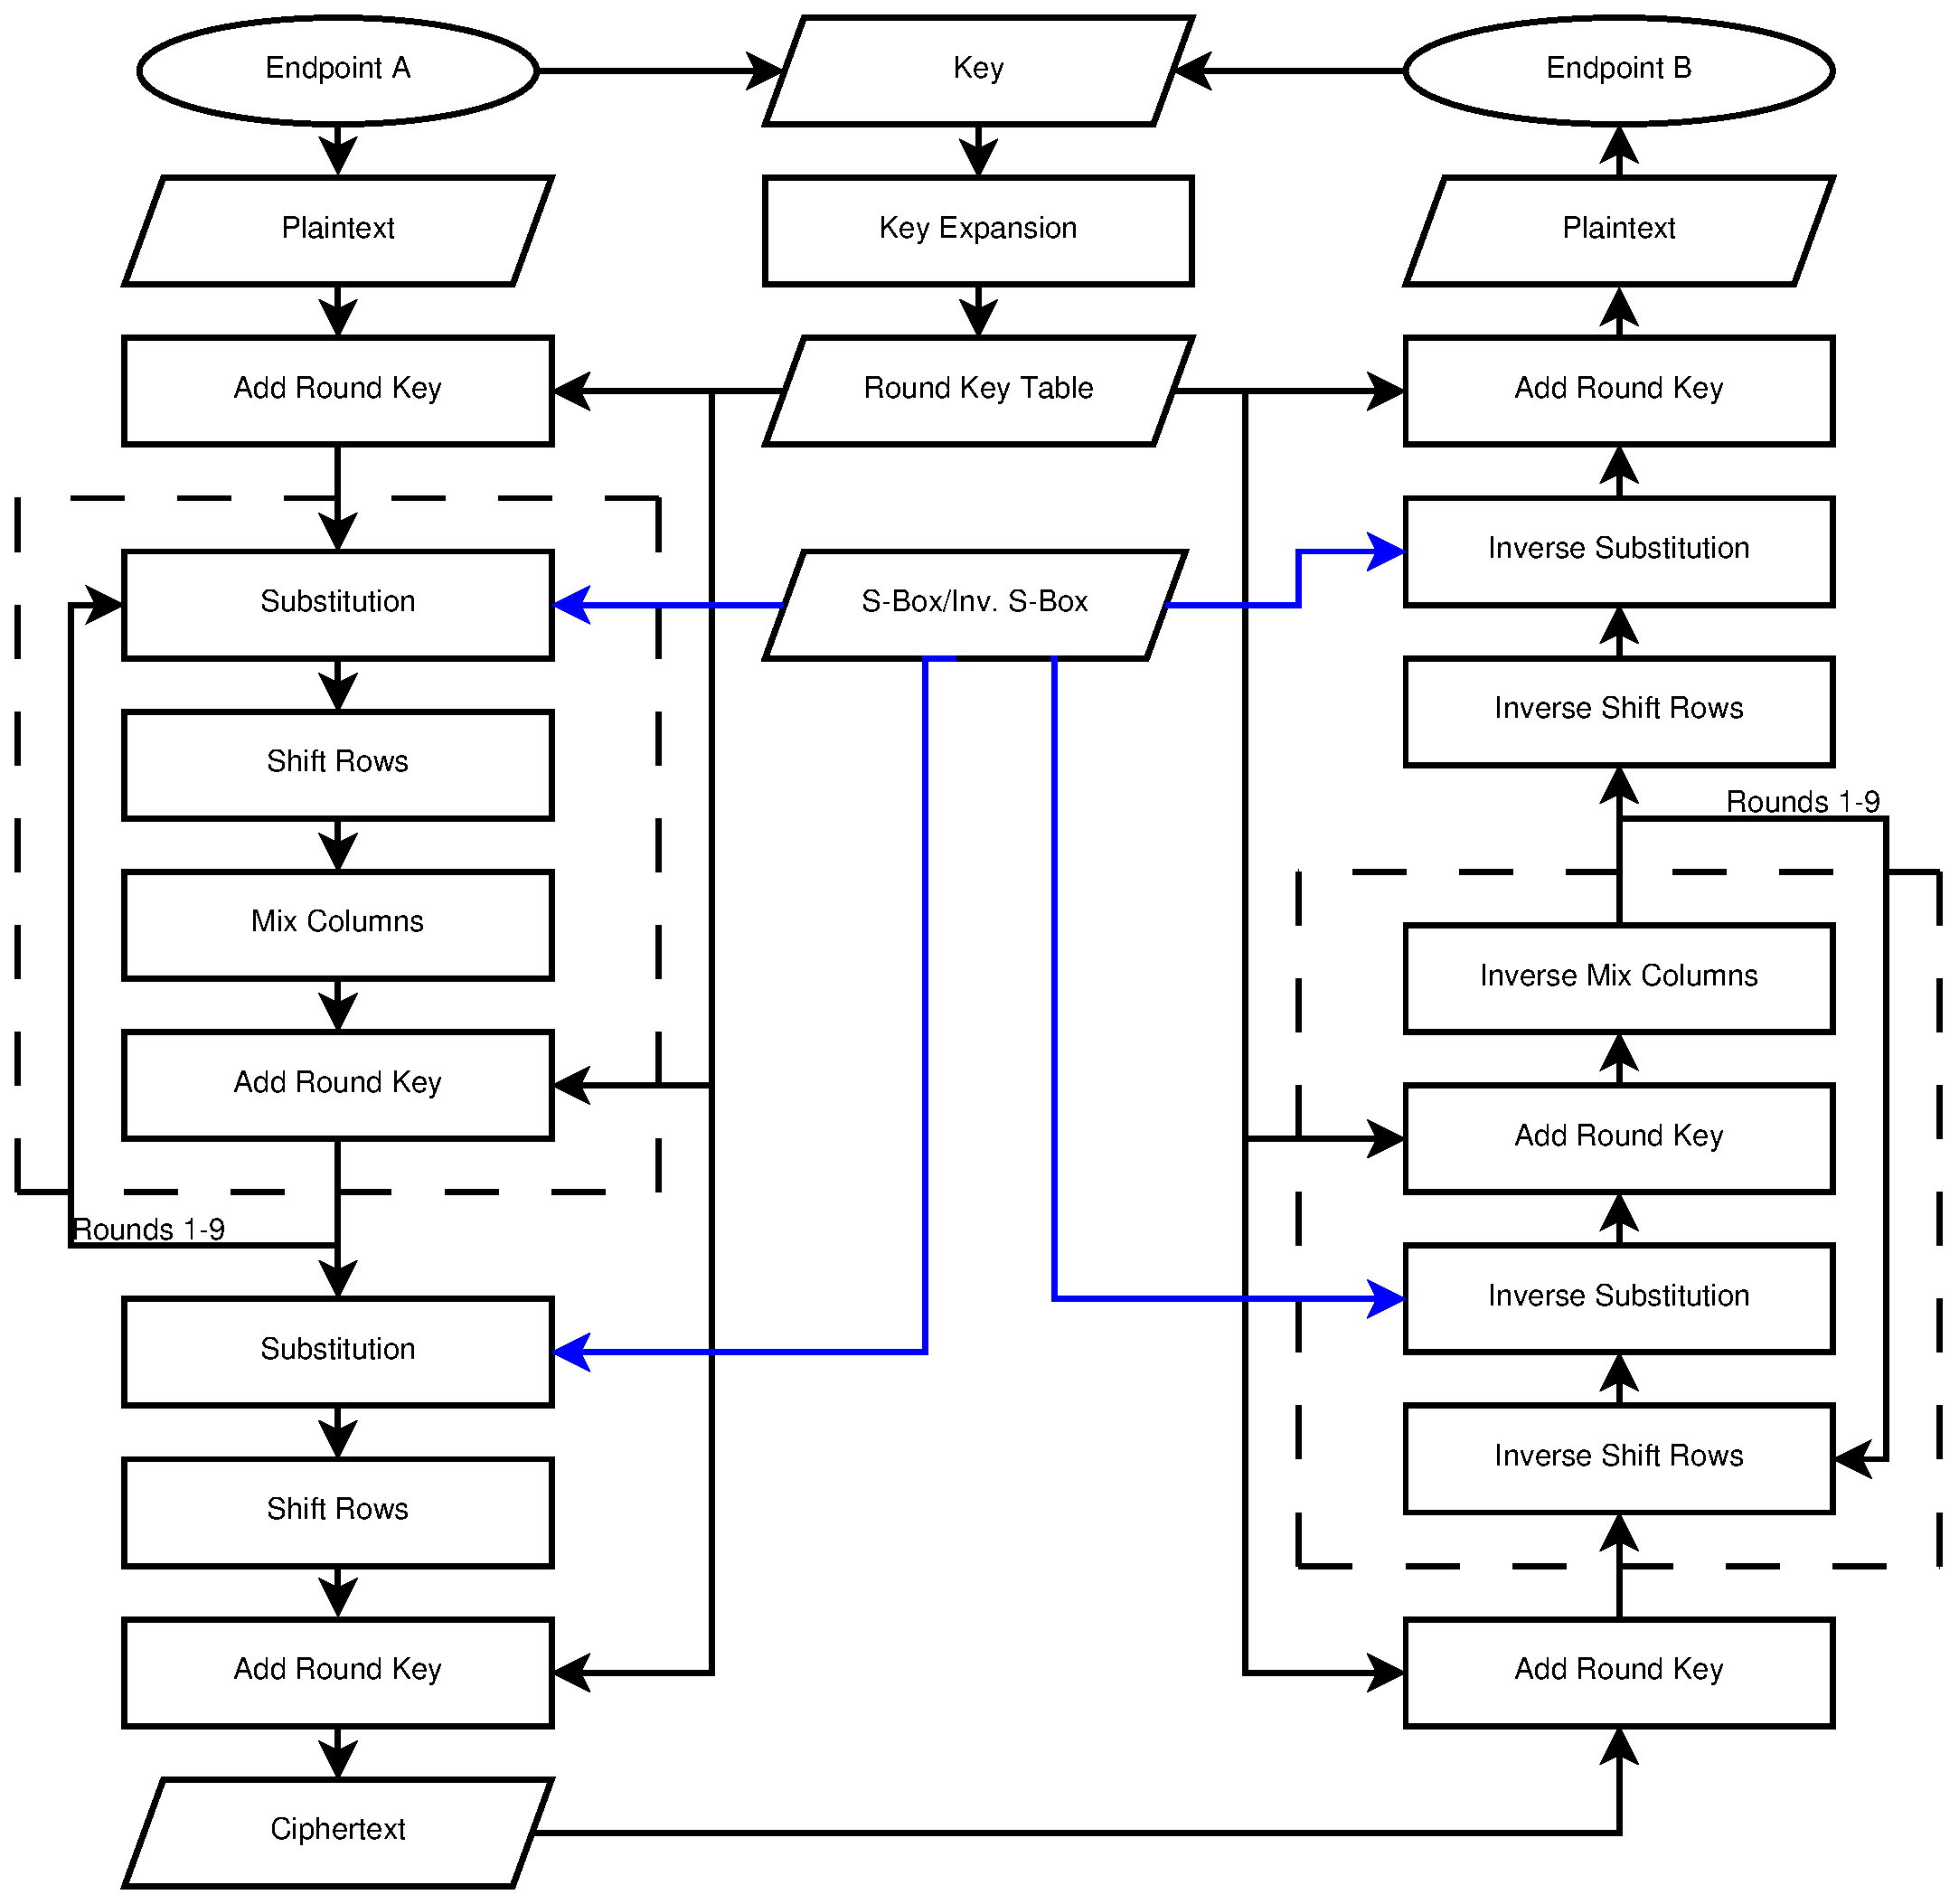
\includegraphics[width=2.5in]{AESProcess}
	\caption{128-Bit AES Process}
	\label{Figure:AESProcess}
\end{figure}
\begin{figure}[!t]
	\centering
	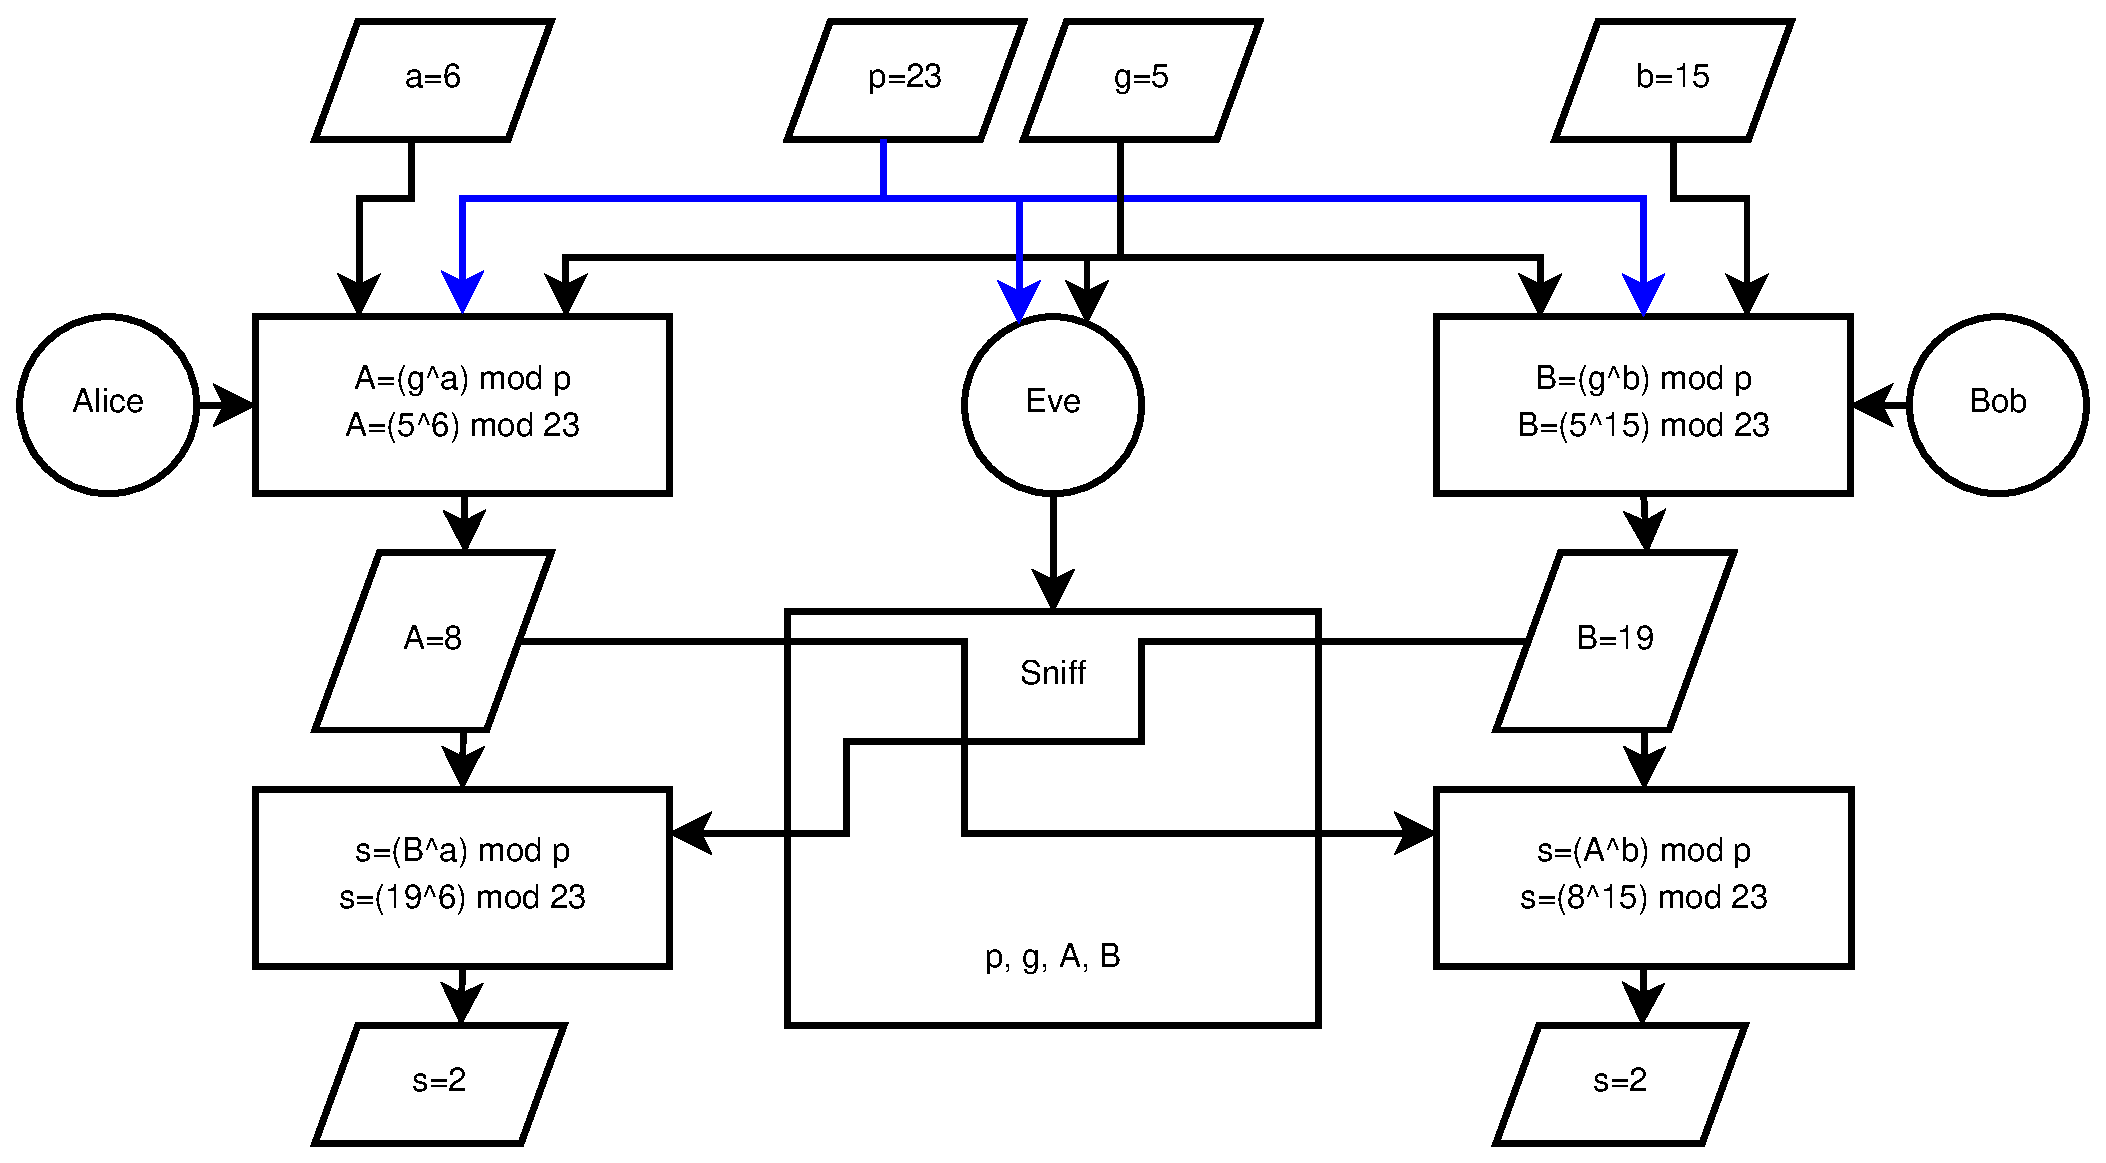
\includegraphics[width=2.5in]{DiffieHellman}
	\caption{Diffie-Hellman Key Exchange}
	\label{Figure:DiffieHellman}
\end{figure}

\section{Related Work}

\cite{AESDynamicKey} Dang, T. N. and H. M. Vo have proposed a method for dynamically modifying the 
shared key based on the frame sequence.

\cite{AESDiffieHellman} Yusfrizal, Y., et al. have proposed a method for exchanging secret keys using
Diffie-Hellman Key Exchange. The shared secret key is used in the AES encryption and decryption.

\cite{AESDynamicSBox} M, G. and H. S. M. have proposed a method for dynamically generating S-Boxes. 
The S-Box is initialized with values from 0 to 255. 256 random numbers are generated and run through 
a hashing algorithm. The resultant hash is stored in a Key matrix. The values of the S-Box are swapped 
based on the Key matrix resulting in a dynamic S-Box. 

\cite{AESKeySBox} Kazys Kazlauskas and Jaunius Kazlauskas have proposed a method for generating S-Boxes dependent on the input key.

\begin{figure}[!t]
	\centering
	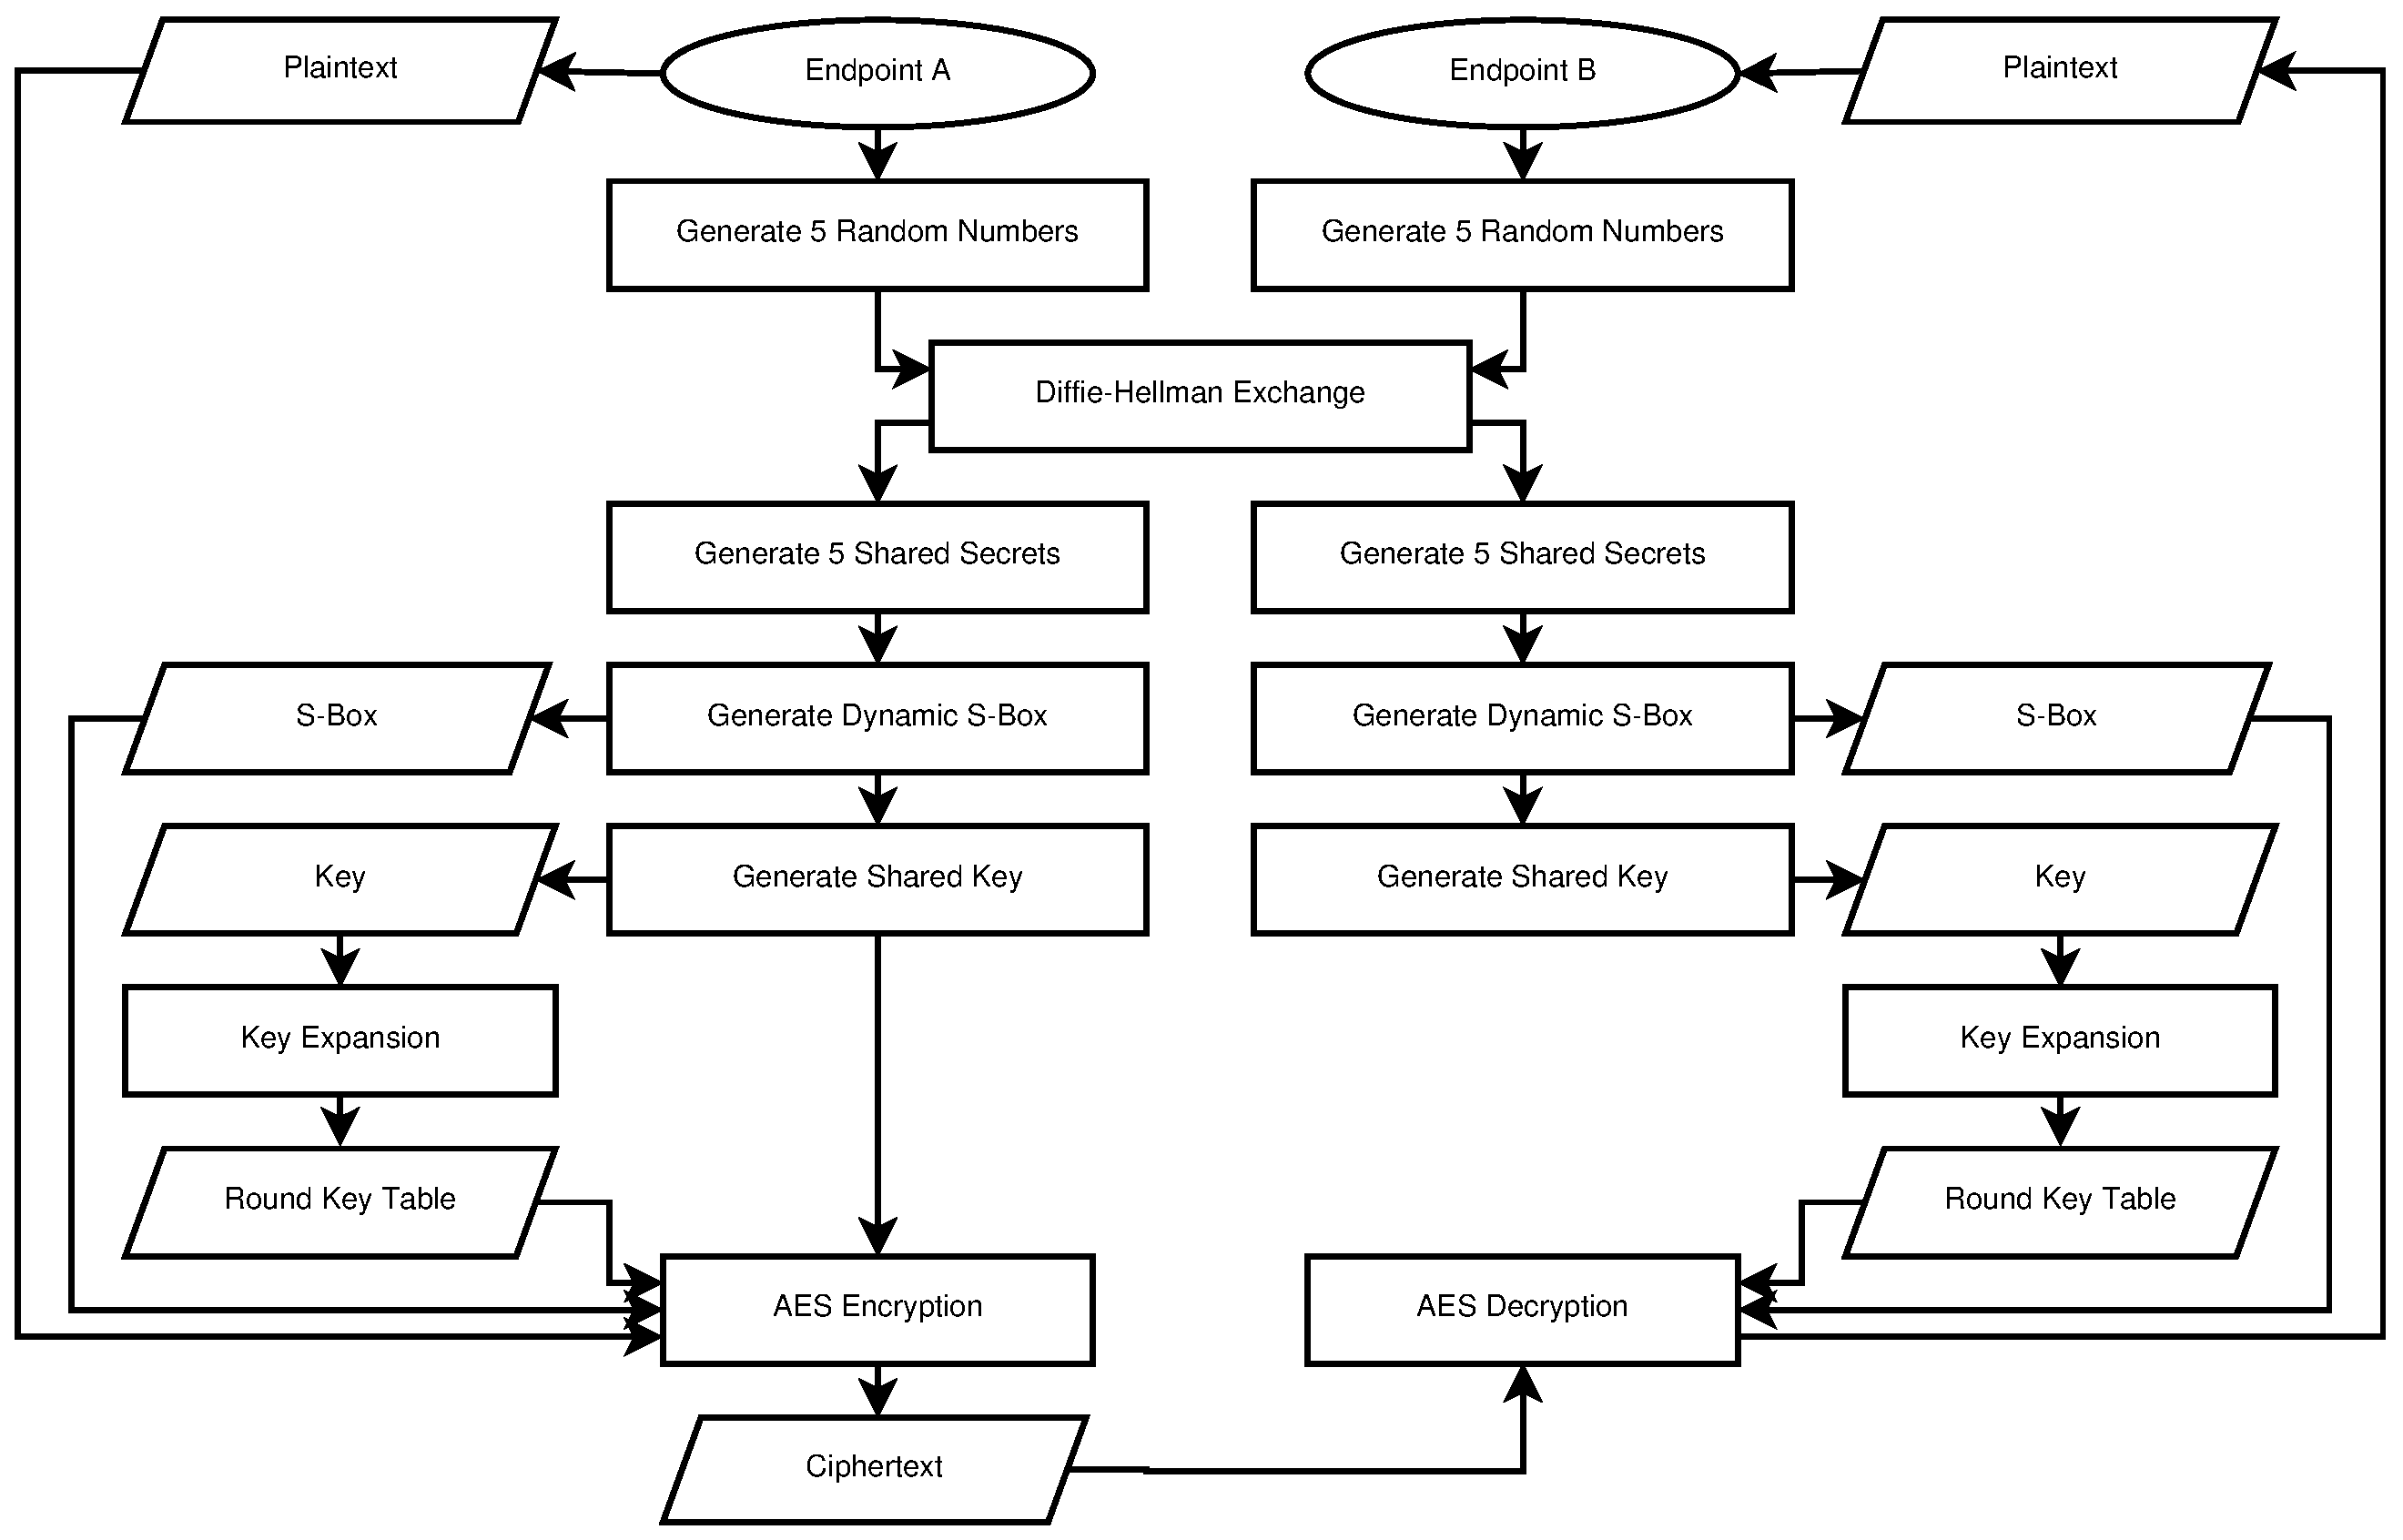
\includegraphics[width=2.5in]{AESDynamicSBox}
	\caption{Dynamic S-Box Generation and Exchange}
	\label{Figure:DynamicSBoxExchange}
\end{figure}

\section{Problem Statement}
While methods exist to exchange keys between endpoints, the S-Box generally remains static. This leaves AES
open to potential exploitation. This paper proposes a method of utilizing Diffie-Hellman Key Exchange coupled
with a Hashing algorithm to generate Shared Secrets which can be used to dynamically generate S-Boxes and 
Inverse S-Boxes.

\section{Dynamic S-Box Generation and Exchange}
In this design, illustrated in Figure ~\ref{Figure:DynamicSBoxExchange}, Diffie-Hellman Key Exchange is combined with Dynamic S-Box Generation to enhance 128-bit AES. Endpoints A and B generate 5 64-bit random numbers. A and B perform Diffie-Hellman Key Exchange to exchange 5 Shared Secrets. Both endpoints calculate and store the SHA-512 hash of each Shared Secret. 128 bits of the first Shared Secret Hash are used as the Secret Key. The remaining 4 Shared Secret Hashes are combined into a 256-Byte array. A and B use the 256-Byte array to dynamically generate the S-Box using the approach described in \cite{AESKeySBox}. This design is implemented in a Visual C++ static library and is illustrated in Figure ~\ref{Figure:CollaborationSession}.

\subsection{Session}
The Session object maintains the private keys, Shared Secrets, and Shared Secret Hashes. This object provides the application with the ability to generate and process Establish Session messages. This object performs the necessary Diffie-Hellman operations to calculate the Shared Secrets from the given private keys and received public keys. 

\subsection{Establish Session Message}
The Establish Session message contains public variables p and g, as well as the Public Key. This object also performs the necessary Diffie-Hellman operations to calculate the Public Key.

\subsection{AES Configuration}
The AES Configuration object maintains the S-Box, Inverse S-Box (I-Box), and the expanded key schedule. This object is capable of generating a Dynamic S-Box and corresponding I-Box from an array of 256 bytes. The Dynamic S-Box generation is based on the approach in \cite{AESKeySBox}. This object uses the 256-Byte array of hash values, instead of the input key, to generate the S-Box and I-Box:
\begin{algorithm}
	\caption{Dynamic S-Box Generation}\label{euclid}
	\begin{algorithmic}[1]
		\Procedure{Generate S-Box}{}
		\State $i \gets 0$
		\State $k \gets 1$
		\State $l \gets 1$
		\State $B \gets \textit{256-Byte Array Of Hashes}$
		\State $S \gets \textit{256 Byte Array of Subtotals}$
		\State $S[0] \gets (B[0]+B[1]) modulo 256$
		\State $SBox[0] \gets S[0]$
		\While{$k<256$}
			\State $i \gets i + 1$
			\State $m \gets 1 + (k+(i*l)) \textit{mod 256}$
			\State $S[i] \gets (S[i-1]+B[m])$
			\State $l \gets 0$
			\For{$j=0;j<k;j \gets j + 1$}
				\If{$\textit{S}[i]!=\textit{SBox}[j]$}
					\State $l \gets l + 1$
				\EndIf	
			\EndFor
			\If{$l==j$}
				\State $SBox[k]=S[i]$
				\State $k \gets k+1$
			\EndIf	
		\EndWhile
		\For{$k=0;k<256;k++$}
			\State $IBox[SBox[k]] \gets k$
		\EndFor
		\EndProcedure
	\end{algorithmic}
\end{algorithm} 

\subsection{Encryptor}
The Encryptor object provides the encryption operation using the given AES Configuration object's S-Box, I-Box, and Key Schedule.

\subsection{Decryptor}
The Decryptor object provides the decryption operation using the given AES Configuration object's S-Box, I-Box, and Key Schedule.

\begin{figure}[!t]
	\centering
	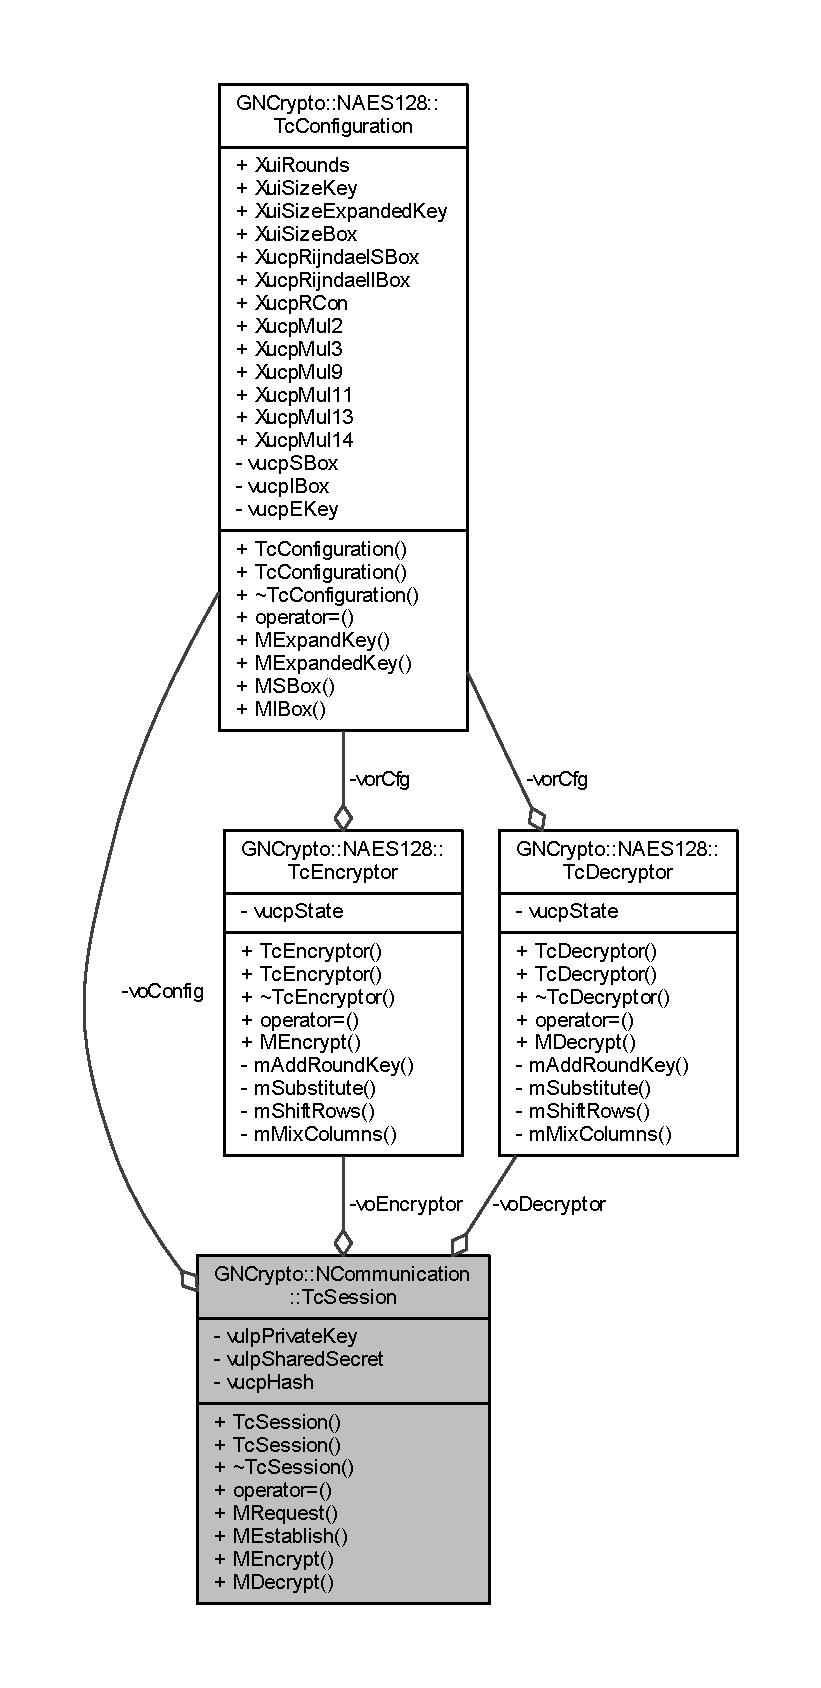
\includegraphics[width=2.5in]{CollaborationSession}
	\caption{Dynamic S-Box Generation and Exchange}
	\label{Figure:CollaborationSession}
\end{figure}

\section{Simulation}
Figure ~\ref{Figure:Sequence} illustrates the Dynamic S-Box Generation and Exchange sequence. Two endpoints are created, Alice and Bob. They each create 5 private keys (64-bit random numbers) then instantiate a Session object, providing the private keys for initialization. Alice initiates a new secure session by creating an Establish Session Message via the Session object, then transmits the message to Bob. Bob's Session object receives the Establish Session Message, calculates 5 Shared Secrets, updates the AES Configuration object with the Shared Secrets, and creates an Establish Session Message containing Bob's Public Key. Bob transmits the Establish Session Message to Alice. Alice's Session object receives the Establish Session Message, calculates 5 Shared Secrets, and updates the AES Configuration object with the Shared Secrets. Alice and Bob can communicate securely using the Encryptor object to encrpt data and the corresponding Decryptor object to decrypt data.

\begin{figure}[!t]
	\centering
	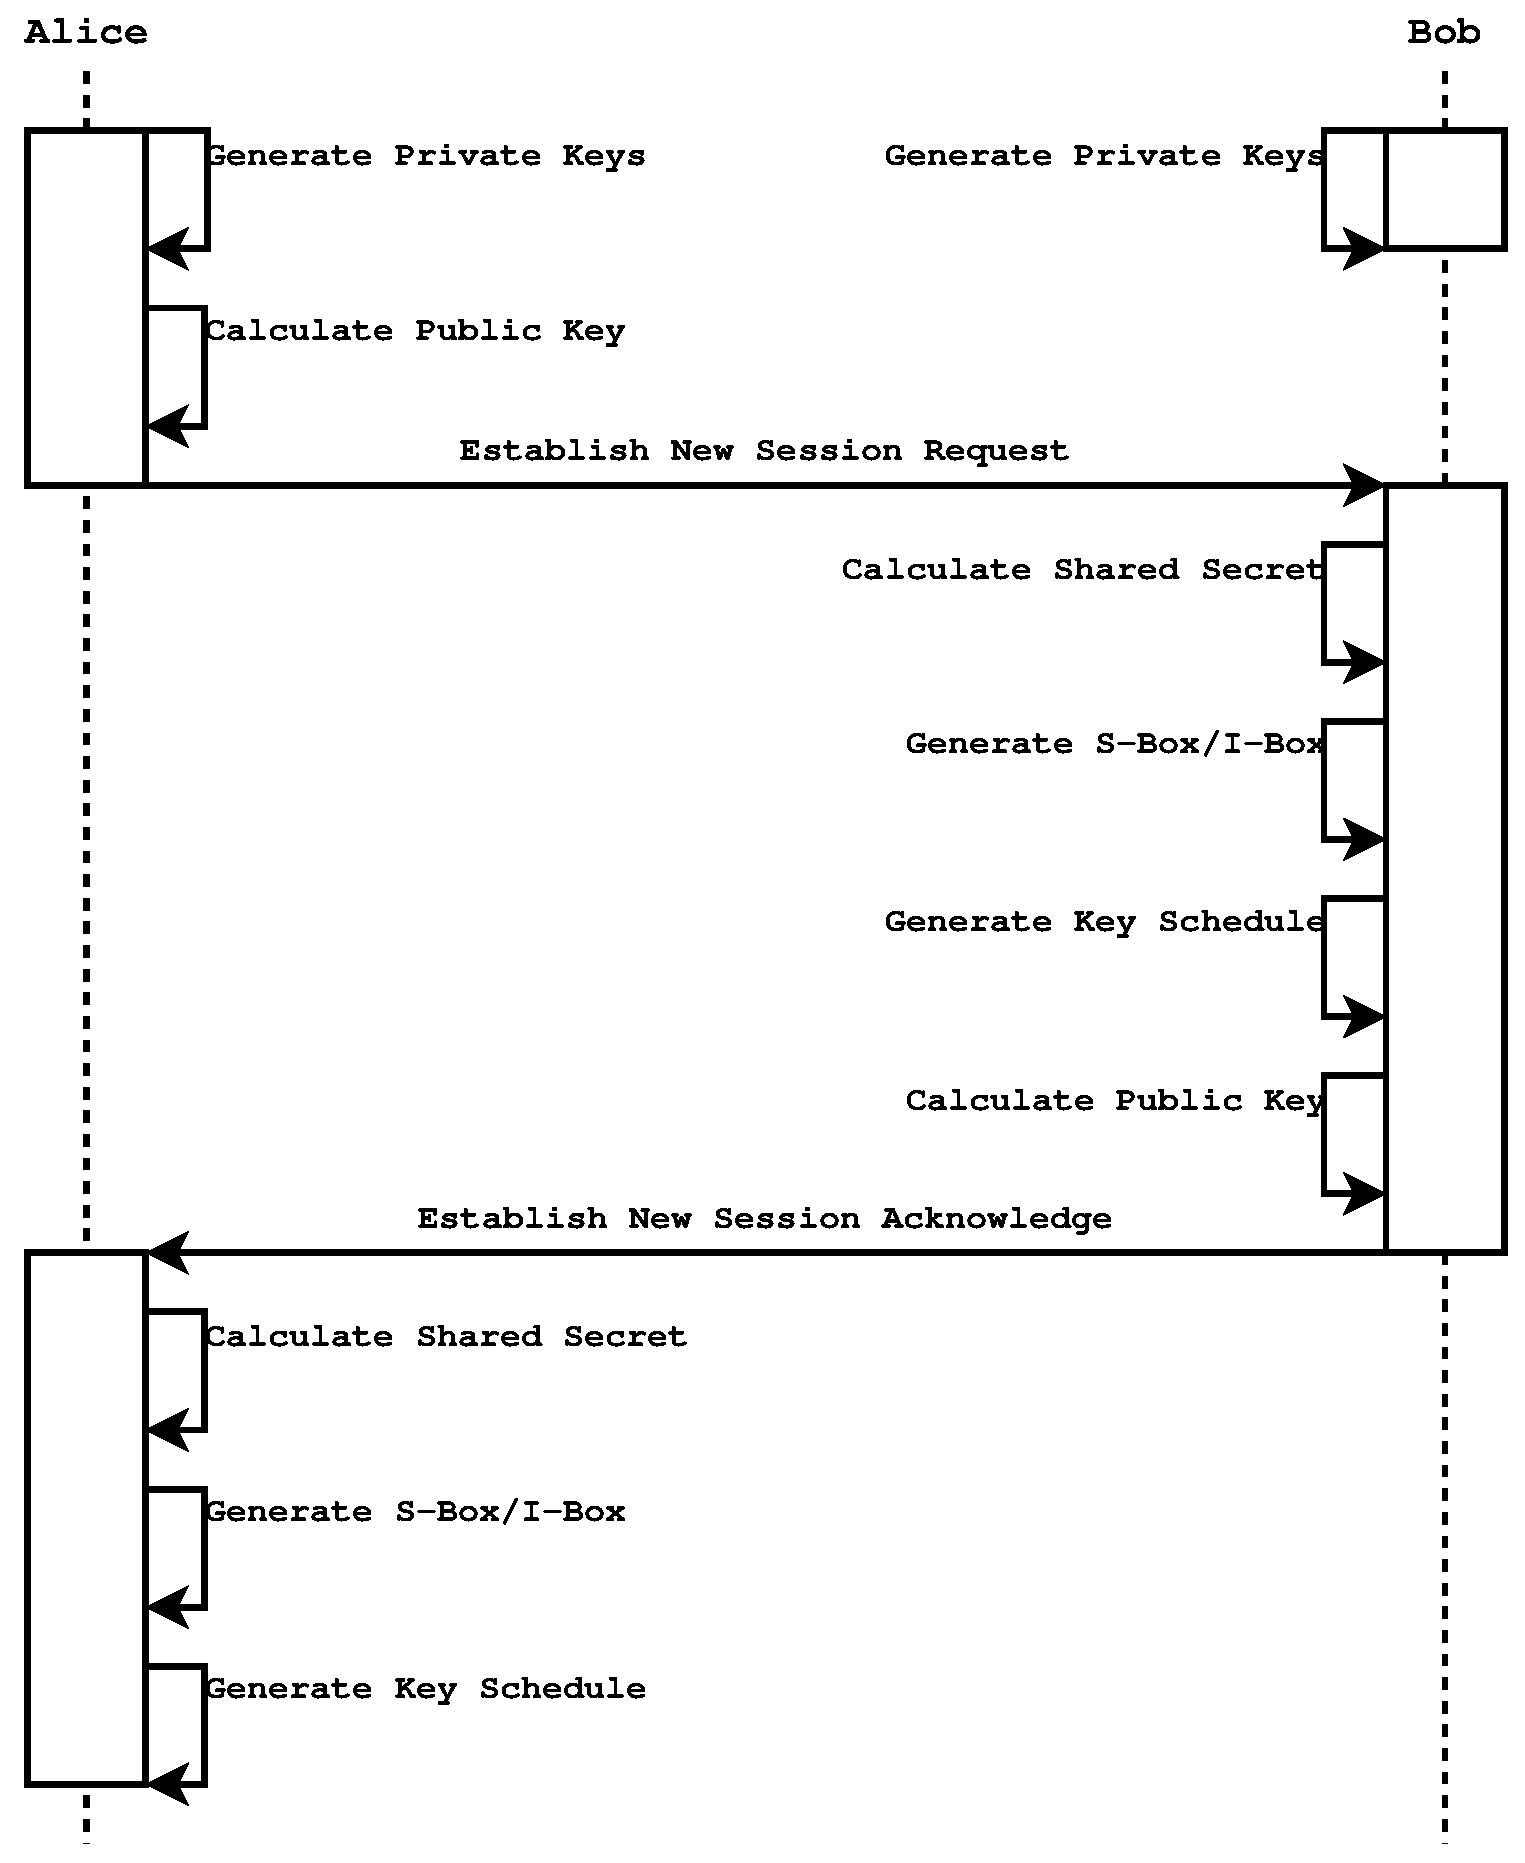
\includegraphics[width=2.5in]{Sequence}
	\caption{Dynamic S-Box Sequence}
	\label{Figure:Sequence}
\end{figure}

\section{Results Analysis and Discussion}
Alice generates the following private keys:
$$
\begin{bmatrix} 
4 & 5 & 6 & 7 & 8
\end{bmatrix}
$$

Bob generates the following private keys:
$$
\begin{bmatrix} 
3 & 4 & 5 & 6 & 7
\end{bmatrix}
$$

Alice and Bob calculate the following Shared Secrets:
$$
\begin{bmatrix}
40 & 5d & 4f & 0c & 5b
\end{bmatrix}
$$

Alice and Bob calculate the following Hash value for Shared Secret 0x40:
$$
\begin{bmatrix}
49 & 0d & 3f & 33 & e4 & e5 & 92 & a7 \\
73 & 7d & 62 & 3d & 31 & cf & e7 & 38 \\
21 & 3f & 82 & b8 & 2d & 35 & b4 & 7d \\
22 & 2b & d2 & a3 & 28 & d2 & b8 & 9d \\
73 & 97 & b2 & 0f & f9 & 1d & 50 & e7 \\
e3 & 70 & f7 & d2 & 05 & aa & 03 & 12 \\
1d & 0b & 68 & fd & 5b & 8a & 20 & 62 \\
4b & cc & 28 & 93 & 1b & 36 & cf & 1a 
\end{bmatrix}
$$

Alice and Bob's AES Configuration object calculates the following Key Schedule from the first 128-bits of the calculated Hash value:
$$
\begin{bmatrix}
49 & 0d & 3f & 33 & e4 & e5 & 92 & a7 \\
73 & 7d & 62 & 3d & 31 & cf & e7 & 38 \\
c2 & 99 & 38 & f4 & 26 & 7c & aa & 53 \\
55 & 01 & c8 & 6e & 64 & ce & 2f & 56 \\
4b & 8c & 89 & b7 & 6d & f0 & 23 & e4 \\
38 & f1 & eb & 8a & 5c & 3f & c4 & dc \\
3a & 90 & 0f & fd & 57 & 60 & 2c & 19 \\
6f & 91 & c7 & 93 & 33 & ae & 03 & 4f \\
d6 & eb & 8b & 3e & 81 & 8b & a7 & 27 \\
ee & 1a & 60 & b4 & dd & b4 & 63 & fb \\
4b & 10 & 84 & ff & ca & 9b & 23 & d8 \\
24 & 81 & 43 & 6c & f9 & 35 & 20 & 97 \\
fd & a7 & 0c & 66 & 37 & 3c & 2f & be \\
13 & bd & 6c & d2 & ea & 88 & 4c & 45 \\
79 & 8e & 62 & e1 & 4e & b2 & 4d & 5f \\
5d & 0f & 21 & 8d & b7 & 87 & 6d & c8 \\
ee & b2 & 8a & 48 & a0 & 00 & c7 & 17 \\
fd & 0f & e6 & 9a & 4a & 88 & 8b & 52 \\
31 & 8f & 8a & 9e & 91 & 8f & 4d & 89 \\
6c & 80 & ab & 13 & 26 & 08 & 20 & 41 \\
37 & 38 & 09 & 69 & a6 & b7 & 44 & e0 \\
ca & 37 & ef & f3 & ec & 3f & cf & b2
\end{bmatrix}
$$


Alice and Bob calculate Hash values for Shared Secrets 0x5d, 0x4f, 0x0c, and 0x5b then combine them into the following 256-byte array:
$$
\begin{bmatrix}
cd & 7b & 83 & 86 & af & b8 & 8b & 6d & fe & 0d \\
5c & 99 & de & ba & 0d & 65 & 3c & 4c & 33 & cd \\
d4 & 71 & 45 & 39 & 0c & b0 & df & aa & 09 & fa \\
80 & b0 & 30 & 9f & c8 & 58 & 5a & fc & 98 & c5 \\
a1 & 81 & d9 & 79 & 18 & 6c & a0 & 31 & 8c & 6b \\
af & 97 & d0 & cb & d6 & 0a & 53 & ee & 57 & 85 \\
b6 & 93 & 13 & ba & 2c & 48 & ac & dc & 4d & 11 \\
f1 & 6f & 65 & 43 & c0 & 8a & d7 & cd & 2c & 0f \\
42 & e7 & 71 & 25 & 39 & bb & 47 & ff & 53 & c3 \\
cf & 27 & 36 & 37 & 24 & bc & f2 & 17 & 90 & 26 \\
99 & 26 & 1e & 38 & 41 & 31 & 31 & 52 & 25 & 63 \\
09 & f3 & 70 & d9 & 72 & 98 & da & 0b & 8a & 0e \\
61 & d6 & 7e & 7b & 3f & 7b & 16 & 33 & 42 & 41 \\
88 & 04 & 01 & 6a & 2b & 15 & d3 & 33 & be & 16 \\
21 & bc & fd & e8 & df & ef & 2a & 2b & 5d & 98 \\
8f & 26 & 58 & 95 & f9 & 3c & d7 & 73 & bc & 51 \\
64 & 39 & bc & 14 & 41 & 5b & ff & ff & 9c & 93 \\
f9 & b1 & c2 & 18 & ba & e1 & 13 & 52 & 70 & 73 \\
9f & 6f & a5 & f3 & 32 & 80 & ba & 52 & 3a & 0a \\
9d & ca & 35 & 03 & 55 & 3d & de & 94 & 9a & 2c \\
7f & 35 & 1e & 65 & 67 & 5b & cf & 0d & e2 & 0d \\
b2 & bc & 07 & 65 & 86 & 87 & c3 & 88 & 52 & 84 \\
99 & e5 & 71 & ac & e9 & 1d & e1 & 8c & 30 & 88 \\
67 & 36 & c3 & e0 & 03 & e6 & 0f & bb & 6f & b3 \\
71 & 97 & 1a & 09 & f4 & 32 & 86 & d1 & ab & cb \\
e6 & df & 0a & 5f & 71 & af
\end{bmatrix}
$$

Alice and Bob pass the 256-Byte array into their AES Configuration objects. The AES Configuration object generates the following S-Box:
$$
\begin{bmatrix} 
48 & ce & 86 & e2 & 2e & 0d & 09 & b8 & 00 & 71 \\
97 & 15 & 04 & fd & 91 & 72 & ed & b5 & c6 & f7 \\
e6 & a0 & 28 & 5b & a3 & d3 & 70 & 64 & 7c & 9a \\
56 & 3f & 6f & ff & fe & 1a & 19 & d5 & 88 & 9b \\
83 & c0 & b2 & e4 & 17 & 20 & 87 & 9f & 9c & b6 \\
3c & b0 & 8f & af & c3 & 08 & 1e & a1 & 1c & a2 \\
3a & 54 & ec & 42 & fc & a8 & 0f & 62 & c9 & 53 \\
51 & aa & df & ae & 34 & 02 & 35 & 06 & da & 14 \\
32 & 65 & 76 & 4a & 73 & 25 & 3b & 2c & 81 & 60 \\
f9 & 5d & 7b & 1b & f1 & 33 & 75 & 3d & c2 & 41 \\
cd & 45 & 6a & 40 & ea & 6d & 8c & b1 & 46 & 8a \\
8d & dc & 7d & f2 & 78 & 03 & 49 & 2f & e7 & 5e \\
ee & d8 & 94 & a4 & 98 & 07 & 43 & 13 & bd & c8 \\
0c & f5 & cc & f8 & 23 & 58 & 66 & bb & 67 & 12 \\
be & 99 & 1f & 84 & d4 & 5c & e0 & 29 & 47 & 31 \\
10 & 44 & bf & 52 & 95 & a6 & 3e & 55 & a9 & 21 \\
82 & de & 68 & b9 & 01 & 96 & 18 & 38 & f4 & b4 \\
5f & fb & ca & d7 & 8e & 2a & 63 & 6e & d6 & 27 \\
b3 & 24 & f3 & 57 & 8b & b7 & d9 & e8 & 61 & 7e \\
7f & 89 & e5 & 79 & 74 & 92 & 93 & 4f & 90 & 37 \\
39 & c7 & 80 & bc & 05 & d2 & f0 & e9 & 69 & 36 \\
77 & d0 & 11 & 0e & a7 & 9e & c1 & 1d & 85 & 4d \\
dd & a5 & cf & 22 & 2b & 59 & 0a & eb & f6 & 4c \\
ab & 16 & 4b & db & d1 & e3 & fa & 6b & 50 & 7a \\
ef & 9d & c5 & ba & 5a & 30 & 4e & cb & 26 & 0b \\
c4 & ad & e1 & ac & 2d & 6c 
\end{bmatrix}
$$

Alice and Bob's AES Configuration object generates the following Inverse S-Box:
$$
\begin{bmatrix} 
08 & a4 & 4b & 73 & 0c & cc & 4d & 7d & 37 & 06 \\
e2 & f9 & 82 & 05 & d5 & 42 & 96 & d4 & 8b & 7f \\
4f & 0b & e7 & 2c & a6 & 24 & 23 & 5d & 3a & d9 \\
38 & 8e & 2d & 9f & df & 86 & b5 & 55 & f8 & b3 \\
16 & 93 & af & e0 & 57 & fe & 04 & 75 & f5 & 95 \\
50 & 5f & 4a & 4c & d1 & c7 & a7 & c8 & 3c & 56 \\
32 & 61 & 9c & 1f & 67 & 63 & 3f & 7e & 97 & 65 \\
6c & 94 & 00 & 74 & 53 & e8 & e5 & db & f6 & c5 \\
ee & 46 & 99 & 45 & 3d & 9d & 1e & b7 & 87 & e1 \\
f4 & 17 & 91 & 5b & 77 & aa & 59 & bc & 43 & b0 \\
1b & 51 & 88 & 8a & a2 & d0 & 66 & ed & ff & 69 \\
b1 & 20 & 1a & 09 & 0f & 54 & c2 & 60 & 52 & d2 \\
72 & c1 & ef & 5c & 1c & 70 & bd & be & ca & 58 \\
a0 & 28 & 8f & da & 02 & 2e & 26 & bf & 6d & b8 \\
6a & 6e & ae & 34 & c6 & 0e & c3 & c4 & 7a & 9a \\
a5 & 0a & 7c & 8d & 1d & 27 & 30 & f1 & d7 & 2f \\
15 & 39 & 3b & 18 & 7b & dd & 9b & d6 & 41 & 9e \\
47 & e6 & fd & fb & 49 & 35 & 33 & 6b & 2a & b4 \\
a9 & 11 & 31 & b9 & 07 & a3 & f3 & 89 & cb & 80 \\
8c & 98 & 29 & d8 & 62 & 36 & fa & f2 & 12 & c9 \\
81 & 44 & ac & f7 & 84 & 64 & 01 & de & d3 & ea \\
cd & 19 & 90 & 25 & b2 & ad & 79 & ba & 4e & e9 \\
6f & dc & a1 & 48 & 92 & fc & 03 & eb & 2b & c0 \\
14 & 76 & bb & cf & 68 & e3 & 3e & 10 & 78 & f0 \\
ce & 5e & 71 & b6 & a8 & 83 & e4 & 13 & 85 & 5a \\
ec & ab & 40 & 0d & 22 & 21 
\end{bmatrix}
$$

Alice encrypts and sends the test string to Bob ("SENDER: Alice $\backslash$r$\backslash$n RECIPIENT: BOB $\backslash$r$\backslash$nSUBJECT: Test Message"). Bob receives the encrypted message and decrypts it into matching plaintext. 

\section{Results Comparison}
The AES-128 test vector uses the following plaintext:

$$
\begin{bmatrix}
00 & 11 & 22 & 33 & 44 & 55 & 66 & 77 \\
88 & 99 & AA & BB & CC & DD & EE & FF
\end{bmatrix}
$$

The AES-128 algorithm using the Rijndael S-Box produces the following ciphertext:
$$
\begin{bmatrix}
69 & c4 & e0 & d8 & 6a & 7b & 04 & 30 \\
d8 & cd & b7 & 80 & 70 & b4 & c5 & 5a
\end{bmatrix}
$$

The AES-128 algorithm using the Dynamic S-Box produces the following ciphertext:
$$
\begin{bmatrix}
 df & c2 & a0 & a4 & ea & cc & 3b & 86 \\
cb & b7 & 5a & 16 & c5 & 7e & c8 & 60
\end{bmatrix}
$$

The AES-128 algorithm using the Rijndael S-Box and the Dynamic S-Box both produce the original plaintext.

\section{Conclusion}
This design proposes a method of dynamically generating S-Boxes and Inverse S-Boxes based on public key exchanged shared secrets. The Dynamic S-Box Generation AES implementation requires additional configuration steps, but eliminates the potential for S-Box exploitation.

\section{Future Work}
This design can be extended to support both the 192-bit and 256-bit versions of AES. The public key exchange can be improved by using the Elliptic-Curve Diffie-Hellman Public Key Exchange. Additionally, this design suffers from man-in-the-middle attacks. This can be mitigated by incorporating public key certificates into the public key exchange.

% if have a single appendix:
%\appendix[Proof of the Zonklar Equations]
% or
%\appendix  % for no appendix heading
% do not use \section anymore after \appendix, only \section*
% is possibly needed

% use appendices with more than one appendix
% then use \section to start each appendix
% you must declare a \section before using any
% \subsection or using \label (\appendices by itself
% starts a section numbered zero.)
%


\appendices
% use section* for acknowledgment
%\section*{Acknowledgment}


% Can use something like this to put references on a page
% by themselves when using endfloat and the captionsoff option.
\ifCLASSOPTIONcaptionsoff
  \newpage
\fi

% trigger a \newpage just before the given reference
% number - used to balance the columns on the last page
% adjust value as needed - may need to be readjusted if
% the document is modified later
%\IEEEtriggeratref{8}
% The "triggered" command can be changed if desired:
%\IEEEtriggercmd{\enlargethispage{-5in}}

% references section

\begin{thebibliography}{1}
  
\bibitem{AESDynamicKey}
Dang, T. N. and H. M. Vo, \emph{Advanced AES Algorithm Using Dynamic Key in the Internet of Things System}.\hskip 1em plus
0.5em minus 0.4em\relax IEEE 4th International Conference on Computer and Communication Systems (ICCCS), 2019.

\bibitem{AESDiffieHellman}
Yusfrizal, Y., et al., \emph{Key Management Using Combination of Diffie–Hellman Key Exchange with AES Encryption}.\hskip 1em plus
0.5em minus 0.4em\relax 6th International Conference on Cyber and IT Service Management (CITSM), 2018.

\bibitem{AESDynamicSBox}
M, G. and H. S. M., \emph{Improved Dynamic S-Box generation using Hash function for AES and its Performance Analysis}.\hskip 1em plus
0.5em minus 0.4em\relax Second International Conference on Green Computing and Internet of Things (ICGCIoT), 2018.

\bibitem{AESKeySBox}
Kazys Kazlauskas and Jaunius Kazlauskas, \emph{Key-Dependent S-Box Generation in AES Block Cipher System}.\hskip 1em plus 0.5em minus 0.4em\relax Informatica, Vol. 20, No. 1, 2009.

\end{thebibliography}

%\begin{IEEEbiographynophoto}{Edward Eisenberger}
%\begin{IEEEbiography}{Edward Eisenberger}
%Biography text here.
%\end{IEEEbiography}


\end{document}


